% ERA-Großpraktikum: Entwickleranleitung -- Allgemeines

\section{Allgemeines}

Diese Sektion ist eine Einführung in die von uns genutzten Entwicklungswerkzeuge,
welche für die Entwicklung des Simulators benötigt werden. Das Ziel dieser Sektion
ist es, dass Leser am Ende in der Lage sind, eigenständig einen Build des Projekts
durchzuführen und somit am Projekt arbeiten können. \\
Des Weiteren wird erläutert, welche Philosophie hinter der Auswahl an Werkzeugen
steckt, von der wir uns erhoffen, dass zukünftige Entwickler diese fortsetzen.

\subsection{Git}
Bei der Entwicklung von Software im Team ist es zwingend notwendig, viele verschiedene Versionen
derselben Software zu verwalten. Deshalb haben wir uns für
\textit{Git}\footnote{\url{https://git-scm.com/}} als Versionskontrollsystem entschieden. \\
Das allein beschreibt allerdings noch nicht, \textit{wie} wir Git verwenden. Daher haben wir uns für
die folgenden Systeme entschieden:

\subsubsection{Gitflow}

\textit{Gitflow}\footnote{\url{https://www.atlassian.com/git/tutorials/comparing-workflows/}} ist
ein beliebtes Modell der Git-Nutzung, welches vor allem bei der Verwaltung von großen Projekten
zum Einsatz kommt. Die von uns genutzte Variante lässt sich wie folgt beschreiben:

\todo[inline]{Ich bin hier schon mal einen Schritt weiter gegangen und hab noch eine Unterscheidung
zwischen dev und master Branch eingefügt. So wollten wir das ja ursprünglich machen, aber aus
Bequemlichkeit nutzen wir nur den master. Falls nach der Abgabe noch Änderungen vorgenommen werden,
sollten wir das dann nach dem "richtigen" Modell machen.}

\begin{itemize}
	\item Es gibt einen \textit{Master}-Branch, der immer die aktuellste, stabile Version enthält.
	\item Es gibt einen \textit{Development}-Branch, der den aktuellen Stand bei der Entwicklung
	einer neuen Version enthält. Der Code ist ebenfalls stabil, wenn auch manche Funktionen noch
	nicht vollständig sein können.
	\item Die einzelnen Aufgaben werden isoliert in einer \textit{Feature}-Branch bearbeitet.
	\item Ist eine Aufgabe fertig, so wird der entsprechende Feature Branch in den Development
	Branch gemerged.
	\item Ist eine neue Version auf dem Development Branch fertiggestellt, so wird die Development
	Branch in den Master Branch gemerged.
\end{itemize}

\subsubsection{Github}

\todo[inline]{Das hier geht schon in Richtung Projektleiterbericht, ich denke es ist aber trzdm sinnvoll,
hier ein paar Worte zu verlieren, da es schließlich zur Entwicklung dazugehört}

Wir nutzen \textit{Github}\footnote{\url{https://github.com/}} as Filehoster des Simulators. Neben
Gründen wie der großen Bekanntheit von Github und der auch für Einsteiger geeigneten grafischen
Oberfläche, sind vor allem folgenden Funktionen hilfreich bei der Entwicklung:

\begin{itemize}
	\item \textit{Issues}: Die im vorherigen Kapitel genannten Aufgaben werden mit einem Issue
	verwaltet. Über die Nummer eines Issues lässt sich der Status der Entwicklung verfolgen.
	\item \textit{Pull Requests}: Nach der Fertigstellung einer Feature Branch wird ein Pull Request
	erstellt, sodass andere Entwickler ein Code Review anfertigen können.
	\item Integration von Tools wie \textit{Waffle}\footnote{\url{https://waffle.io/}} und
	\textit{Travis CI}\footnote{\url{https://travis-ci.org/}}
\end{itemize}

\subsection{C++}

Der Simulator ist zum Großteil in C++ geschrieben. Unser Augenmerk liegt dabei auf Portabilität
zwischen verschiedenen Compilern, weshalb wir uns auf den \textbf{C++14} Standard geeinigt haben,
sowie möglichst wenige externe Bibliotheken verwenden.

\subsubsection{Compiler}

Wir arbeiten mit folgenden Compilern:

\begin{itemize}
	\item \textit{g++ $\geq$ 5}
	\item \textit{clang++ $\geq$ 3.7}
\end{itemize}

\subsubsection{Bibliotheken}

Die einzige, für das Endprodukt benötigte Abhängigkeit ist \textit{Qt}\footnote{\url{https://www.qt.io/}}
$\geq$ 5.6 in Kombination mit QtQuick $\geq$ 2.6. Wir verwenden Qt zur Erstellung der grafischen Oberfläche,
haben aber grundsätzlich eine strikte Trennung zwischen Code der GUI und dem Rest des Simulators.
Durch diese Trennung wäre es möglich, den Simulator auch ohne Qt zur Verfügung zu stellen, z.B.
mit einer anderen Grafikbibliothek oder als Kommandozeilenprogramm. \\
Eine Ausnahme zu dieser Trennung bildet die Internationalisierung des Simulators. Der Simulator ist
in der aktuellen Version ausschließlich in Englisch verfügbar, uns war es aber ein großes Anliegen,
auch andere Sprachen unterstützen zu können. Somit verwenden wir die von Qt zur Verfügung gestellten
Mittel, Nutzer sichtbare Nachrichten übersetzbar zu machen, auch in allen anderen Modulen außerhalb
der GUI. So können z.B. Prozessorarchitektur-spezifische Fehlermeldungen übersetzt werden.

\subsubsection{Code Style}

Da der Code nicht nur funktionieren, sondern auch gewissen Standards folgen
sollte, haben wir uns entschieden, den \textit{Google C++ Style Guide}
\footnote{\url{https://google.github.io/styleguide/cppguide.html}} als Grundlage
für unseren Code Style zu nutzen. Folgende Ausnahmen haben wir dabei festgelegt:

\begin{itemize}
	\item Präfix \texttt{\_}, anstatt Suffix \texttt{\_} für private Klassenattribute,
	\item \texttt{.hpp} und \texttt{.cpp} als Dateiendungen für C++ Header/Klassen,
	\item \texttt{camelCase} für Funktionsnamen und
	\item Parameter Namen werden immer angegeben, egal ob benötigt oder nicht.
\end{itemize}

Um dies automatisiert zu gewährleisten, nutzen wir das Tool \textit{ClangFormat}
\footnote{\url{http://clang.llvm.org/docs/ClangFormat.html}}. Damit werden
z.B. Einrückungen automatisch angeordnet. \\
Die Konfiguration von ClangFormat befindet sich in der Datei \texttt{.clang-format}

\subsubsection{Dokumentation}

Neben diesem Bericht ist der gesamte Quellcode des Simulators in Form von
\textit{Doxygen}\footnote{\url{http://www.stack.nl/~dimitri/doxygen/}} Kommentaren
dokumentiert. Diese Dokumentation ist weitaus ausführlicher als dieser Bericht und
ist essentiell für die Weiterentwicklung des Simulators. Neben der einfachsten
Möglichkeit, die Kommentare im Quellcode zu lesen, ist es mit Doxygen ebenfalls möglich,
eine HTML bzw. \LaTeX Version zu generieren. Dazu wechselt man in das \texttt{docs/}
Verzeichnis und führt den Befehl \texttt{doxygen} aus, welcher anschließend die
Dokumentation generiert.

\subsection{Build Umgebung}

Möchte man den Simulator selbst kompilieren, so wird eine Build Umgebung vorausgesetzt.
Wie bereits genannt, liegt unser Augenmerk auf Portabilität zwischen Betriebssystemen,
deshalb wird in dieser Sektion gezeigt, wie man eine solche Umgebung unter den gängigen
Betriebssystemen (Linux, macOS, Windows) einrichten kann.

\subsubsection{Linux}

Da wir eine relativ neu Versionen von Qt verwenden, ist eine reine Installation der
Abhängigkeiten über die Paketverwaltung nur unter solchen Linux Distributionen möglich,
die auch die entsprechenden Versionen in den Paketquellen beinhalten. Während dies unter
Rolling Release Systemen (wie z.B. Arch Linux) ein geringeres Problem ist, haben Anwender von
z.B. Debian basierter Betriebssysteme häufiger mit älterer Software zu kämpfen.
Unter Debian selbst sind die benötigten Versionen erst ab Debian Stretch (Debian 9)
verfügbar, unter Ubuntu erst ab Ubuntu 16.10.

\begin{itemize}
	\item \textbf{Debian basierte Betriebssysteme:} \\
	\todo[inline]{Funktioniert nicht in Ubuntu 16.*}
	\begin{lstlisting}
apt install build-essential cmake git qtdeclarative5-dev
	\end{lstlisting}

	\item \textbf{Arch Linux:} \\
	\begin{lstlisting}
pacman -S base-devel cmake git qt5-declarative \
 qt5-graphicaleffects qt5-quickcontrols
	\end{lstlisting}
\end{itemize}

Ist eine Installation über die Paketquellen nicht möglich, bietet es sich an, Qt manuell
zu installieren\footnote{\url{https://wiki.qt.io/Install_Qt_5_on_Ubuntu}}. Dafür lädt
man sich von der offiziellen Website einen Installer runter, der nach dem Start einen
Installationsort erfragt. Dieser muss später beim Bauen des Projekts angegeben werden.

\subsubsection{Aufsetzen von QtCreator}

QtCreator ist eine integrierte Entwicklungsumgebung, die von Qt selbst zur Verfügung gestellt wird und somit alle Features von Qt (qml, Widget-Designer, ...) nativ unterstützt. Da die IDE auch C++-Programmierung unterstützt, eignet sie sich als Alrounder-IDE für dieses Projekt.\\

Im Folgenden wird das Aufsetzen von QtCreator und erste Schritte danach für \textbf{Ubuntu 16.10} beschrieben:\\

\textbf{QtCreator installieren}\\
Über den Paketmanager:
\begin{lstlisting}
apt install qtcreator
\end{lstlisting}

\textbf{Repository klonen}\\
Siehe \autoref{dev-report-cmake-build}. Endet die Ausführung von cmake in einem Fehler (``Could not find a package configuration file provided by Qt5Widgets``), dann ist vermutlich bei der Installation von \texttt{qtdeclarative5-dev} etwas schiefgegangen.\\

\textbf{In QtCreator CMake-Projekt einrichten}\\
Im Startbildschirm ``Open Project`` und dann die oberste \texttt{CMakeLists.txt} (die in \texttt{era-gp-sim/CMakeLists.txt}) öffnen.\\
Im Reiter ''Configure Project'' für das Kit ''Desktop'' -> Details: Nur Debug und Release anhaken und die Build-Ordner anpassen\footnote{Es bietet sich an, für die IDE einen anderen Build-Ordner zu verwenden, als für das Bauen über die Konsole. Ein CMake-Projekt in QtCreator wird mit CodeBlocks erzeugt und erstellt daher leicht andere Konfigurationsdateien als cmake über die Konsole. Damit beides parallel nebeneinander betrieben werden kann, sollten die Build-Ordner getrennt werden.}. Die Auswahl bestätigen.\\
Jetzt sollte das Edit-Tab mit dem Projekt geöffnet sein. Im unteren Rand unter ''General Messages'' sollte einmal cmake automatisch aufgerufen worden sein, links oben im ''Projects'' Fenster sollte die Struktur des Projekts (mit CMakeLists.txt, include, source, tests und third-party) zu sehen sein.\\
Im Projects-Tab (linker Rand, Schraubenschlüssel) im Reiter ''Build \& Run'' wird jetzt der Build-Prozess konfiguriert.
Bei ''Edit build configuration'' Debug auswählen, dann unter ''Build Steps'' folgendes verändern:\\
\includegraphics[scale=0.5]{images/setup-qtcreator-build-config.png}\\
Der Eintrag von cmake Arguments soll dabei der relative Pfad vom eingetragenen Build-Ordner zum obersten Ordner des Projekts sein. Im Beispiel ist der Build-Order unter \texttt{era-gp-sim/build\_qtcreator\_debug} angelegt, d.h. eine Ebene höher liegt der root-Ordner des Projekts. Das \texttt{-j4} Argument bei \texttt{make} erhöht die Geschwindigkeit beim Bauen, da 4 Jobs gleichzeitig ausgeführt werden.
Zur Run-Konfiguration wechseln 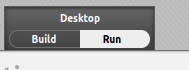
\includegraphics[scale=1.0]{images/setup-qtcreator-run-config.png} und als ''Working Directory'' den Build-Ordner eintragen.\\

Nun zurück wechseln und bei ''Edit build configuration'' Release auswählen und sowohl ''Build Steps'' als auch ''Run'' wie oben verändern.\\

Ins Edit-Tab wechseln und am linken Rand unten beim Monitor von ''Release'' auf ''Debug'' wechseln und dann mit Klick auf den Hammer das Projekt bauen.\\
\includegraphics[scale=0.7]{images/setup-qtcreator-change-build-flavor.png}\\
Hier können dann auch später statt ''era-sim'' verschiedene Test-Suits lokal ausgeführt werden. In der ''Compile Output'' Konsole kann der Fortschritt des Bauvorgangs überwacht werden.\\


\textbf{Nützliche Einstellungen}\\
\begin{itemize}
	\item File Naming:\\
	Im Menü \texttt{Tools -> Options}, dort in der linken Auswahlliste C++ -> Reiter ''File Naming'':\\
	Bei Headers Suffix zu hpp ändern.
	\item Lizenz automatisch einfügen:\\
	Im Menü \texttt{Tools -> Options -> C++ -> FileNaming}: Unter ''License Template'' kann der Pfad zu einer Textdatei eingegeben werden, deren Inhalt dann als Kommentar an den Anfang jeder neu erzeugten Datei platziert wird.
	\item Auto-Formatting (Plugin):\\
	 Muss evtl. über \texttt{Help -> About plugins} herunterladen (''Beautifier''). Ist dann unter \texttt{Tools -> Options -> Beautifier} zu finden.
\end{itemize}

\textbf{Erste Schritte}\\
\begin{itemize}
	\item Neue Datei erstellen:\\
	\texttt{File -> New File or Project}
	\item Aktuelle Datei formatieren:\\
	\texttt{Tools -> Beautifier -> ClangFormat -> Format Current File}
\end{itemize}



\subsubsection{macOS}

\textbf{Qt installieren}

Um Qt auf ein Mac-Computer zu installieren, bietet es sich an, den Installer zu
verwenden, den man über die offizielle Website herunterladen kann
\footnote{\url{https://www.qt.io/download/}}. Bei der Installation können neben der
aktuellsten auch ältere Versionen des Framework heruntergeladen werden. Nach
der Installation befindet sich am angegebenen Installationspfad ein Ordner "Qt",
in dem sich auch der QtCreator-IDE befindet.

\textbf{CMake aktualisieren}

Zum Bauen des Projekts wird CMake benötigt, das in der Regel über einen
Paketmanager installiert oder alternativ von der offiziellen Website
heruntergeladen werden kann.

\textbf{In QtCreator CMake-Projekt einrichten}

Um ein CMake-Projekt in QtCreator einzurichten, können die selben Schritte, wie
im Kapitel für Linux beschrieben, durchgeführt werden.

\subsubsection{Windows}

Unter Windows ist es ähnlich wie unter macOS: Die Installation von Qt ist mit
einem Installer am angenehmsten, wobei es sich anbietet, die Open Source Version
von Qt zu verwenden. Des Weiteren haben wir die besten Erfahrungen mit MinGW
\footnote{\url{http://www.mingw.org/}} gemacht, da der Qt Installer anbietet,
dies automatisch zu installieren. Schließlich wird noch CMake benötigt, was man
sich von der offiziellen Website herunterlädt. \\
Mit QtCreator ist der Einrichtungsaufwand am geringsten, da etwaige Pfade zu
Bibliotheken automatisch eingerichtet werden. Die Einrichtung entspricht den
selben Schritten, wie im Kapitel für Linux.

Unter Windows gibt es zugegebenermaßen die meisten Probleme, da viele kleine
Faktoren mitspielen. Bei Problemen sollte die Suchmaschine der Wahl, oder gleich
eine virtuelle Maschine mit einem Linux für die Entwicklung verwendet werden.

\subsection{CMake / Make}
\label{dev-report-cmake-build}
Um auch den Build Prozess unabhängig vom Betriebssystem durchzuführen, haben wir uns für
\textit{CMake}\footnote{\url{https://cmake.org/}} entschieden. CMake generiert die benötigten
\texttt{Makefiles} für jedes Betriebssystem bzw. jeden Compiler neu, welche anschließend
von \textit{Make}\footnote{\url{https://www.gnu.org/software/make/}} ausgeführt werden können.

Um einen Build des Projekts durchzuführen, sollte vorher einen entsprechende Build Umgebung
aufgesetzt werden. Anschließend kann man mit den Folgenden Befehlen einen Clean Build erzeugen:

\begin{lstlisting}[language=bash, keywords={}]
# Projekt herunterladen
git clone https://github.com/TUM-LRR/era-gp-sim

# In das Projektverzeichnis wechseln
cd era-gp-sim

# Submodule initialisieren (Google Test)
git submodule update --init

# Build Verzeichnis erstellen und betreten
mkdir build && cd build

# Mit CMake die Makefiles erzeugen
cmake ..

# Projekt bauen (Die Option -j setzt Anzahl an
# Jobs und beschleunigt so den Build Prozess)
make -j 4

# Programm starten
./bin/era-sim
\end{lstlisting}

Hat man Qt manuell installiert, ist es ggf. notwendig, den Installationspfad bei der
Ausführung von CMake zu spezifizieren.

\begin{lstlisting}[language=bash, keywords={}]
# Wurde z.B. der Ordner ~/Qt5.7.0 bei der manuellen
# Installation von Qt angegeben, so muss man CMake mit
# dem folgenden Argument aufrufen:
cmake -D CMAKE_PREFIX_PATH=~/Qt5.7.0/5.7/gcc_64 ..
\end{lstlisting}

Alternativ ist es auch möglich, mit der von Qt mitgelieferten Entwicklungsumgebung
\textit{QtCreator}\footnote{\url{https://wiki.qt.io/Qt_Creator}} zu arbeiten.
Dabei öffnet man die \texttt{CMakeLists.txt} als Projekt, und hat so eine grafische
Oberfläche für die Entwicklung am Simulator. Auch CMake/Make muss so nicht mehr
manuell über die Kommandozeile bedient werden, ein Build kann über die grafische
Oberfläche von QtCreator erzeugt werden.

\subsection{Tests}

Wir nutzten das \textit{Google Test}\footnote{\url{https://github.com/google/googletest}} Framework
zur Automatisierung unserer Tests. Die Tests befinden sich im \texttt{tests/} Verzeichnis, gruppiert
nach ihren Modulen. Da Tests der grafischen Oberfläche zu komplex wären, haben wir uns auf die übrigen
Module des Simulators beschränkt, deren korrekte Funktionalität in jeweils separaten Unit Tests
überprüft wird.

Um ein einheitliches Ergebnis bei den Tests zu erzielen, nutzen wir das Continuous Integration Tool
\textit{Travis CI}\footnote{\url{https://travis-ci.org/}}. Dabei wird nach jedem hoch geladenen
Commit ein Clean Build angefertigt, der alle verfügbaren Tests durchführt. Das Ergebnis dieses Tests
wird auf Github veröffentlicht und ist bindend. Die Tests werden sowohl mit g++, als auch mit clang
durchgeführt. \\
Die Konfiguration von Travis befindet sich in der Datei \texttt{.travis.yml}

Die Tests können auch lokal ausgeführt werden. Dazu wechselt man mit \texttt{cd} in das Build
Verzeichnis und nutzt das von CMake mitgelieferte Programm \texttt{ctest} um die Tests zu starten.
Um die Testgeschwindigkeit zu erhöhen empfiehlt es sich, mit der \texttt{-j} Option die Anzahl
der Jobs zu erhöhen.

\subsection{Projektstruktur}

In diesem Kapitel wird die Funktion jedes Ordners beschrieben.

\begin{itemize}
	\item \textbf{\texttt{docs/}} enthält die Dokumentation von \erasim, also
	die Berichte und die Konfiguration von Doxygen.
	\item \textbf{\texttt{examples/}} enthält Beispielprogramme für RISC-V.
	\item \textbf{\texttt{include/}} enthält alle C++ Header Dateien, gruppiert
	nach ihrem Modul. Wir haben uns um die strikte Trennung zwischen Header- und
	Source Dateien bemüht.
	\item \textbf{\texttt{isa/}} enthält die Architekturdefinitionen in YAML und
	JSON Konfigurationsdateien.
	\item \textbf{\texttt{scripts/}} enthält für die Entwicklung nützliche
	Skripte, um z.B. neue Klassen zu erstellen (inklusive Header- und
	Source Datei).
	\item \textbf{\texttt{source/}} enthält C++ Source Dateien, ebenfalls
	gruppiert nach ihren Modulen. Auch hier sei auf die strikte Trennung
	zwischen Header- und Source Dateien verwiesen.
	\item \textbf{\texttt{tests/}} enthält die Unit Tests jeder Module.
	\item \textbf{\texttt{third-party/}} enthält genutzte Bibliotheken. Konkret
	wird Google Tests dadurch eingebunden und ein JSON Parser bereitgestellt.
\end{itemize}